\qcor targets an execution model whereby application execution is directed by the host with access to an attached quantum device. Applications are broadly thought of as containing two components: a main, classical part, and one or more quantum kernels or subroutines. Figure \ref{fig:exec_model} illustrates \qcor's execution model. Designated quantum kernels are compiled and offloaded to the quantum device. The quantum device executes \qcor library calls and/or \qcor regions identified by directive notations. When the host encounters a quantum kernel, in the form of compiled quantum instructions, the kernel is passed asynchronously to the quantum device controller.
% Execution on the host is asynchronous to execution on the quantum device. 
\qcor exposes initialization, synchronization, execution, and memory management library \ac{API}s to the user that enable a wide variety of hybrid quantum-classical use cases.

\begin{figure*}
 \centering
 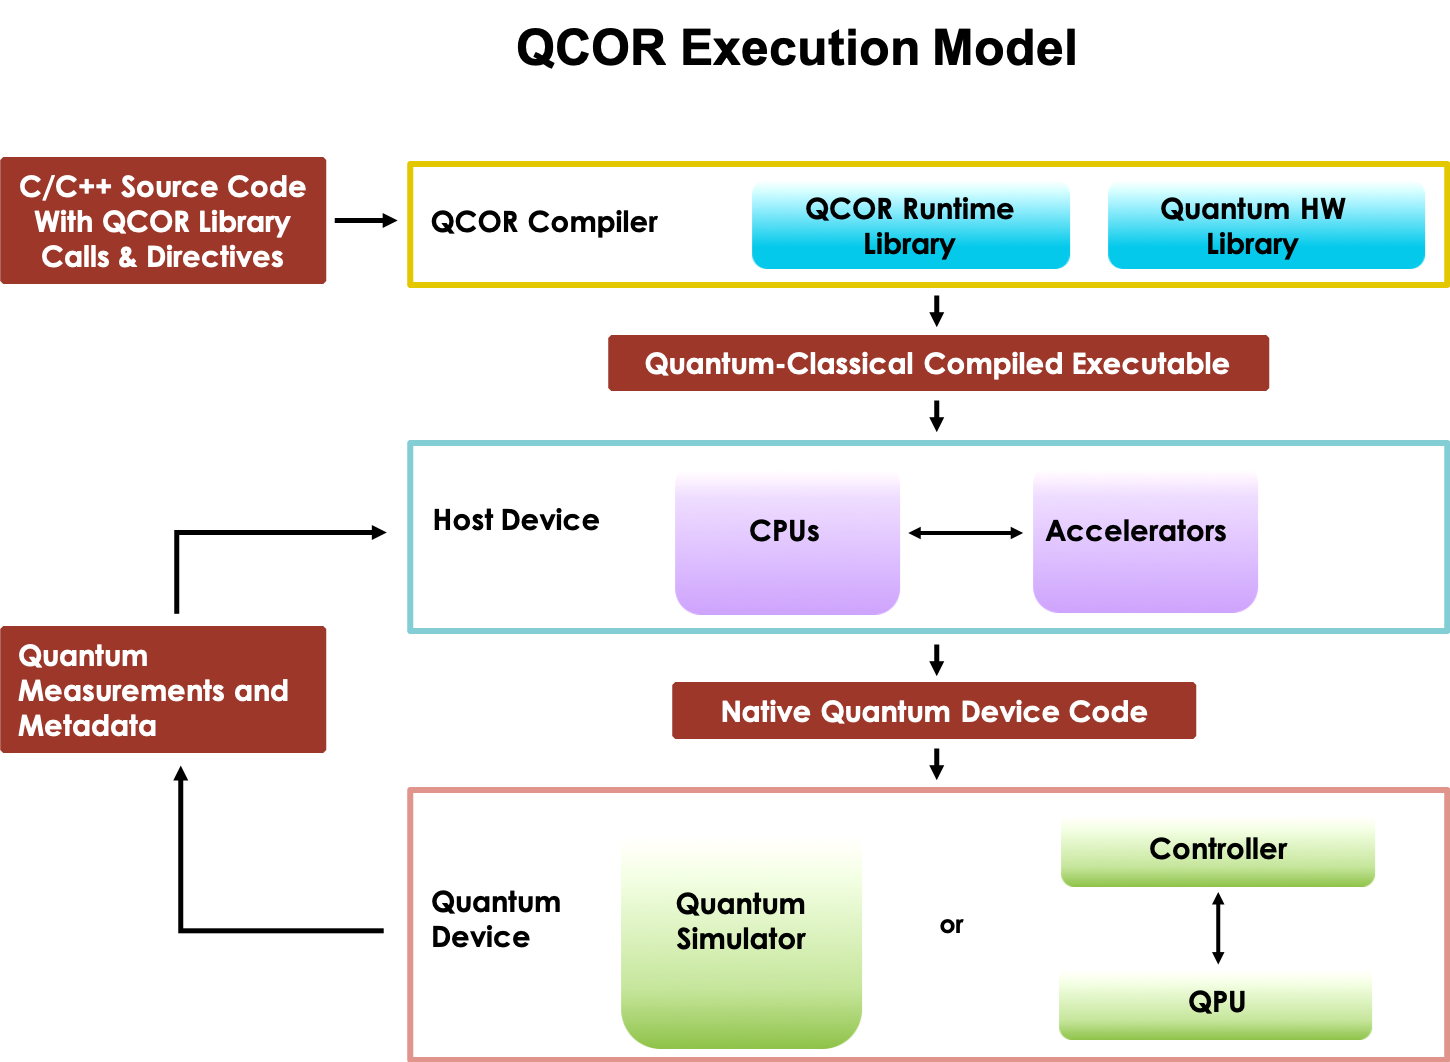
\includegraphics[width=5in,height=4in]{figures/Execution_Model_Illustration_v3.png}
  \caption{Diagram of \qcor Execution Model}
  \label{fig:exec_model}
\end{figure*}


\subsection{\textbf{Quantum Kernels}}\label{subsec:kernel}
\qcor extends \CorCpp by allowing the programmer to define functions, called \FUNC{kernels}, that, when called, are executed asynchronously on the quantum device. A \FUNC{kernel} is defined using the \_\_qpu\_\_ declaration specifier. A \FUNC{kernel} can optionally include a \qcor \DATATYPENAME{Observable} and a list of other native or user defined \CorCpp datatypes.

The \FUNC{kernel} function body should be a sequence of instructions on qbits and can also include control flow statements and predefined macros.  This circuit level expressiveness can be implemented using languages like \textit{QASM}, \textit{XASM}, and \textit{Quill}. 
%TODO: Insert footnotes or citations for qasm, xasm and quill

The sample code below illustrates \FUNC{kernel} usage in a \CorCpp program.
%TODO: insert example
